\begin{figure}[t]
\centering
\begin{tikzpicture}
\begin{axis}[
  width=0.72\textwidth,
  height=0.58\textwidth,
  axis equal image,
  xlabel={$\eta_1$},
  ylabel={$\eta_2$},
  xmin=-0.56,
  xmax=1.04,
  ymin=-0.56,
  ymax=1.04,
  grid=both,
  minor tick num=1,
  legend style={at={(0.02,0.02)},anchor=south west,draw=none,fill=white},
]
\addplot[
  draw=gray!80,
  fill=gray!30,
  line width=0.5pt,
] coordinates {
  (1,1)
  (0.5,-0.5)
  (-0.5,0.1)
} \closedcycle;
\addlegendentry{all covariant channels}

\addplot[
  table/x index=0,
  table/y index=1,
  draw=orange!85!black,
  fill=orange!55,
  fill opacity=0.58,
  line width=0.6pt,
] table {generated/spin1_positive_polygon.dat} \closedcycle;
\addlegendentry{nonnegative spectrum}

\addplot[
  table/x index=0,
  table/y index=1,
  draw=green!45!black,
  fill=green!55!black,
  fill opacity=0.48,
  line width=0.8pt,
] table {generated/spin1_markov_polygon.dat} \closedcycle;
\addlegendentry{embeddable closure}

\addplot[only marks,mark=*,mark size=1.5pt] coordinates {(1,1)};
\end{axis}
\end{tikzpicture}
\caption{Spin \(1\).  The gray triangle is the exact covariant-channel
simplex.  The orange polygon is its intersection with
\(\eta_1,\eta_2\geq0\).  The green region is the closure of the
covariantly embeddable set and is bounded by
\(\eta_2=\eta_1^3\) and \(\eta_2=\eta_1^{3/5}\), the two extreme rays
of the logarithmic generator cone; \((0,0)\) itself is not a finite-time
endpoint.}
\label{fig:spin-one-regions}
\end{figure}

\begin{figure}[t]
\centering
\begin{minipage}[t]{0.48\textwidth}
\centering
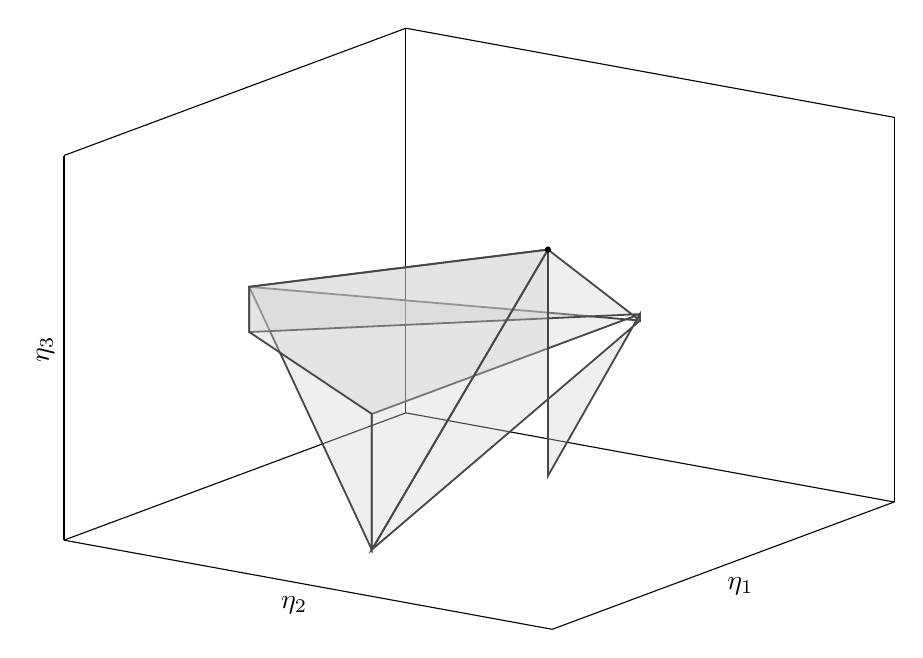
\begin{tikzpicture}
\begin{axis}[
  width=\linewidth,
  height=0.76\linewidth,
  view={125}{22},
  xlabel={\(\eta_1\)},
  ylabel={\(\eta_2\)},
  zlabel={\(\eta_3\)},
  xmin=-0.65,xmax=1.05,
  ymin=-0.65,ymax=1.05,
  zmin=-0.65,zmax=1.05,
  ticks=none,
]
\addplot3[draw=black!72,fill=gray!38,fill opacity=0.34,line width=0.65pt,forget plot] coordinates {
  (-0.6,0.2,-0.0285714285714)
  (0.2,-0.6,0.2)
  (0.733333333333,0.2,-0.6)
} \closedcycle;
\addplot3[draw=black!72,fill=gray!38,fill opacity=0.34,line width=0.65pt,forget plot] coordinates {
  (-0.6,0.2,-0.0285714285714)
  (1,1,1)
  (0.2,-0.6,0.2)
} \closedcycle;
\addplot3[draw=black!72,fill=gray!38,fill opacity=0.34,line width=0.65pt,forget plot] coordinates {
  (-0.6,0.2,-0.0285714285714)
  (0.733333333333,0.2,-0.6)
  (1,1,1)
} \closedcycle;
\addplot3[draw=black!72,fill=gray!38,fill opacity=0.34,line width=0.65pt,forget plot] coordinates {
  (0.2,-0.6,0.2)
  (1,1,1)
  (0.733333333333,0.2,-0.6)
} \closedcycle;

\addplot3[only marks,mark=*,mark size=0.9pt] coordinates {(1,1,1)};
\end{axis}
\end{tikzpicture}

\small (a) all channels
\end{minipage}
\begin{minipage}[t]{0.48\textwidth}
\centering
\begin{tikzpicture}
\begin{axis}[
  width=\linewidth,
  height=0.76\linewidth,
  view={125}{22},
  xlabel={\(\eta_1\)},
  ylabel={\(\eta_2\)},
  zlabel={\(\eta_3\)},
  xmin=0,xmax=1.05,
  ymin=0,ymax=1.05,
  zmin=0,zmax=1.05,
  ticks=none,
]
\addplot3[draw=cbOrange!85!black,fill=cbOrange,fill opacity=0.27,line width=0.65pt,forget plot] coordinates {
  (0,0,0.238095238095)
  (0,0.5,0.357142857143)
  (1,1,1)
  (0.5,0,0.5)
} \closedcycle;
\addplot3[draw=cbOrange!85!black,fill=cbOrange,fill opacity=0.27,line width=0.65pt,forget plot] coordinates {
  (0,0.333333333333,0)
  (0.833333333333,0.5,0)
  (1,1,1)
  (0,0.5,0.357142857143)
} \closedcycle;
\addplot3[draw=cbOrange!85!black,fill=cbOrange,fill opacity=0.27,line width=0.65pt,forget plot] coordinates {
  (0.5,0,0.5)
  (1,1,1)
  (0.833333333333,0.5,0)
  (0.555555555556,0,0)
} \closedcycle;
\addplot3[draw=cbOrange!85!black,fill=cbOrange,fill opacity=0.27,line width=0.65pt,forget plot] coordinates {
  (0,0,0)
  (0,0.333333333333,0)
  (0,0.5,0.357142857143)
  (0,0,0.238095238095)
} \closedcycle;
\addplot3[draw=cbOrange!85!black,fill=cbOrange,fill opacity=0.27,line width=0.65pt,forget plot] coordinates {
  (0,0,0)
  (0,0,0.238095238095)
  (0.5,0,0.5)
  (0.555555555556,0,0)
} \closedcycle;
\addplot3[draw=cbOrange!85!black,fill=cbOrange,fill opacity=0.27,line width=0.65pt,forget plot] coordinates {
  (0,0,0)
  (0.555555555556,0,0)
  (0.833333333333,0.5,0)
  (0,0.333333333333,0)
} \closedcycle;

\addplot3[only marks,mark=*,mark size=0.9pt] coordinates {(1,1,1)};
\end{axis}
\end{tikzpicture}

\small (b) nonnegative spectrum
\end{minipage}
\par\medskip
\begin{minipage}[t]{0.48\textwidth}
\centering
\begin{tikzpicture}
\begin{axis}[
  width=\linewidth,
  height=0.76\linewidth,
  view={125}{22},
  xlabel={\(\eta_1\)},
  ylabel={\(\eta_2\)},
  zlabel={\(\eta_3\)},
  xmin=0,xmax=1.05,
  ymin=0,ymax=1.05,
  zmin=0,zmax=1.05,
  ticks=none,
]
\addplot3[draw=cbOrange!85!black,fill=cbOrange,fill opacity=0.27,line width=0.65pt,forget plot] coordinates {
  (0,0,0.238095238095)
  (0,0.5,0.357142857143)
  (1,1,1)
  (0.5,0,0.5)
} \closedcycle;
\addplot3[draw=cbOrange!85!black,fill=cbOrange,fill opacity=0.27,line width=0.65pt,forget plot] coordinates {
  (0,0.333333333333,0)
  (0.833333333333,0.5,0)
  (1,1,1)
  (0,0.5,0.357142857143)
} \closedcycle;
\addplot3[draw=cbOrange!85!black,fill=cbOrange,fill opacity=0.27,line width=0.65pt,forget plot] coordinates {
  (0.5,0,0.5)
  (1,1,1)
  (0.833333333333,0.5,0)
  (0.555555555556,0,0)
} \closedcycle;
\addplot3[draw=cbOrange!85!black,fill=cbOrange,fill opacity=0.27,line width=0.65pt,forget plot] coordinates {
  (0,0,0)
  (0,0.333333333333,0)
  (0,0.5,0.357142857143)
  (0,0,0.238095238095)
} \closedcycle;
\addplot3[draw=cbOrange!85!black,fill=cbOrange,fill opacity=0.27,line width=0.65pt,forget plot] coordinates {
  (0,0,0)
  (0,0,0.238095238095)
  (0.5,0,0.5)
  (0.555555555556,0,0)
} \closedcycle;
\addplot3[draw=cbOrange!85!black,fill=cbOrange,fill opacity=0.27,line width=0.65pt,forget plot] coordinates {
  (0,0,0)
  (0.555555555556,0,0)
  (0.833333333333,0.5,0)
  (0,0.333333333333,0)
} \closedcycle;

\addplot3[
  surf,
  shader=flat,
  draw=green!35!black,
  line width=0.08pt,
  fill opacity=0.32,
  mesh/rows=33,
] table {generated/spin3_markov_face_1.dat};
\addplot3[
  surf,
  shader=flat,
  draw=green!35!black,
  line width=0.08pt,
  fill opacity=0.32,
  mesh/rows=33,
] table {generated/spin3_markov_face_2.dat};
\addplot3[
  surf,
  shader=flat,
  draw=green!35!black,
  line width=0.08pt,
  fill opacity=0.32,
  mesh/rows=33,
] table {generated/spin3_markov_face_3.dat};
\addplot3[only marks,mark=*,mark size=0.9pt] coordinates {(1,1,1)};
\end{axis}
\end{tikzpicture}

\small (c) embeddable closure within (b)
\end{minipage}
\caption{Spin \(3/2\).  Panels (a) and (b) are generated from exact
rational polytope vertices.  Panel (c) overlays the three green
embeddable-boundary surfaces on the orange nonnegative-spectrum
polytope.  Each surface is obtained by setting one canonical rate to
zero and uses the other rates in \([0,8]\), while the defining cone is
unbounded.}
\label{fig:spin-three-halves-regions}
\end{figure}
